\documentclass[10pt]{article}
\usepackage{fullpage}
\usepackage{amsmath}
\usepackage[amsthm, thmmarks]{ntheorem}
\usepackage{amssymb}
\usepackage{graphicx}
\usepackage{enumerate}
\usepackage{verse}
\usepackage{tikz}
\usepackage{verbatim}
\usepackage{hyperref}
\usepackage{bbm}

\newtheorem{lemma}{Lemma}
\newtheorem{theorem}[lemma]{Theorem}
\newtheorem{definition}[lemma]{Definition}
\newtheorem{proposition}[lemma]{Proposition}
\newtheorem{corollary}[lemma]{Corollary}
\newtheorem{claim}[lemma]{Claim}
\newtheorem{example}[lemma]{Example}

\newcommand{\dee}{\mathrm{d}}
\newcommand{\Dee}{\mathrm{D}}
\newcommand{\In}{\mathrm{in}}
\newcommand{\Out}{\mathrm{out}}
\newcommand{\pdf}{\mathrm{pdf}}
\newcommand{\Cov}{\mathrm{Cov}}
\newcommand{\Var}{\mathrm{Var}}

\newcommand{\ve}[1]{\mathbf{#1}}
\newcommand{\ves}[1]{\boldsymbol{#1}}
\newcommand{\mrm}[1]{\mathrm{#1}}
\newcommand{\etal}{{et~al.}}
\newcommand{\sphere}{\mathbb{S}^2}
\newcommand{\modeint}{\mathcal{M}}
\newcommand{\azimint}{\mathcal{N}}
\newcommand{\ra}{\rightarrow}
\newcommand{\mcal}[1]{\mathcal{#1}}
\newcommand{\X}{\mathcal{X}}
\newcommand{\Y}{\mathcal{Y}}
\newcommand{\Z}{\mathcal{Z}}
\newcommand{\x}{\mathbf{x}}
\newcommand{\y}{\mathbf{y}}
\newcommand{\z}{\mathbf{z}}
\newcommand{\tr}{\mathrm{tr}}
\newcommand{\sgn}{\mathrm{sgn}}
\newcommand{\diag}{\mathrm{diag}}
\newcommand{\Real}{\mathbb{R}}
\newcommand{\sseq}{\subseteq}
\newcommand{\ov}[1]{\overline{#1}}
\newcommand{\data}{\mathrm{data}}
\newcommand{\mtt}[1]{\mathtt{#1}}

\DeclareMathOperator*{\argmin}{arg\,min}
\DeclareMathOperator*{\argmax}{arg\,max}        


\title{DiffusionNet}
\author{Pramook Khungurn}

\begin{document}
\maketitle

This article is written as I read the ``DiffusionNet'' paper by Sharp \etal~\cite{Sharp:2022:DiffusionNet}.

\section{Introduction}

\begin{itemize}
  \item The goal of this paper is to design a neural network architecture for a data type that is not commonly used in mainstream deep learning: points sampled from a surface.
  
  \item There have been multiple attempts at this problem, but they are remaining problems.
  \begin{itemize}
    \item Existing solutions are tied to a particular representation (e.g., triangle meshes or point clouds).
    \item Mesh-based architectures do not scale well to high-resolution surface data. That is, performance degrades if the mesh is refined.
    \item Existing approaches are too sensitive to underlying mesh structure.    
  \end{itemize}

  \item The paper proposes a solution that is both scalable and robust to sampling changes.
  
  \item Main observation.
  \begin{itemize}
    \item Diffusion (i.e., evolution according to the heat equation) is highly effective for spatial communication.
    \item Spatial gradient can be used to capture anisotropy.
  \end{itemize}    

  \item The code for this paper is available at \url{https://github.com/nmwsharp/diffusion-net}.
\end{itemize}

\section{Method}

\begin{itemize}
  \item The method has three building blocks.
  \begin{enumerate}
    \item Multi-layer perceptrons (MLPs) applied at each point independently to model point-wise scalar functions of feature channels.
    \item A learned diffusion operation for propagating information across the domain.
    \item Local spatial gradient features to expand the network's filter space beyond radially symmetric features.
  \end{enumerate}
\end{itemize}

\subsection{Point-Wise MLPs}

\begin{itemize}
    \item As input we are given either a mesh or a point cloud with $V$ vertices.
    \item Each vertex comes with a feature vector of dimension $D$.
    \item The MLP in question is a function $f: \Real^D \ra \Real^D$, which is applied independently at every vertex to transform the feature.
    \item Because the MLP is applied independently to every point, it does not capture spatial structure of the surface.
\end{itemize}


\subsection{Learned Diffusion}

\subsubsection{Background}

\begin{itemize}
    \item To review the Laplacian, see my notes~\cite{Khungurn:Laplacians}.

    \item Let $u(t, \ve{x})$ where $t \in \Real$ and $\ve{x} = (x_1, x_2, \ldots, x_d) \in \Real^d$ be a time-dependent scalar field on a $\Real^d$.
    
    \item {\bf Diffusion} is the process of evolving $u(t, \ve{x})$ according to the {\bf heat equation}:
    \begin{align*}
        \frac{\partial u}{\partial t} = \Delta u
    \end{align*}
    where $\Delta u$ is the {\bf Laplacian} of $u$; that is,
    \begin{align*}
        \Delta u = \sum_{i=1}^d \frac{\partial^2 u}{\partial x_i^2}.
    \end{align*}
    
    \item In particular, $\Delta u(t,\ve{x})$ indicates the difference between the value $u(t,\ve{x})$ and the average value of $u$ in the neighborhood of $\ve{x}$.
    \begin{itemize}
        \item If $\Delta u(t,\ve{x}) > 0$, then $u(t,\ve{x})$ is lower than the average value of $u$ in the neighborhood of $\ve{x}$.
        \item If $\Delta u(t,\ve{x}) < 0$, then $u(t,\ve{x})$ is greater than the average value of $u$ in the neighborhood of $\ve{x}$.
        \item If $\Delta u(t,\ve{x}) = 0$, then $u(t,\ve{x})$ is equal to the average value of $u$ in the neighborhood of $\ve{x}$.
    \end{itemize}

    \item So, evolution according to the heat equation is a smoothing process.
    \begin{itemize}
        \item If $\Delta u(t,\ve{x}) > 0$, then $u(t,\ve{x})$ gets increased.
        \item If $\Delta u(t,\ve{x}) < 0$, then $u(t,\ve{x})$ gets decreased.
        \item If $\Delta u(t,\ve{x}) = 0$, then $u(t,\ve{x})$ is unchanged.
    \end{itemize}
    If we let $u(t,\ve{x})$ evolve over time, peaks will be flattened, and depressions will be filled.\\
    $u$ will tend towards a constant function, whose value is the average of $u$ over the domain.

    \item We call the process ``diffusion'' because information from various parts of the domain must travel to other parts in order for the system to be able to compute the average.
    
    \item The paper says that using the heat equation ensures that the results are largely invariant to the way the surface is sampled or meshed.
    \begin{itemize}
        \item This is because propagation depends only on the domain size and the passage of time, not on how the domain is sampled.
    \end{itemize}
\end{itemize}

\subsubsection{Discretization of the Laplacian}

\begin{itemize}
    \item To perform computation with a computer, one must replace $\Delta$ with matrices. 
    
    \item There are two matrices involved.
    \begin{itemize}
        \item The {\bf weak Laplace matrix} $L \in \Real^{V \times V}$ is positive semi-definite and sparse.
        \item The {\bf mass matrix} $M \in \Real^{V \times V}$ is a diagonal matrix.
    \end{itemize}

    \item The paper follows the convention that the signs of the mass matrix should be such that
    \begin{align*}
        M^{-1}L \approx -\Delta.
    \end{align*}

    \item On triangle meshes, we can use the cotan-Laplace matrix \cite{Crane:DdgCourse:2025}.
    \begin{itemize}
        \item Let there be $T$ triangles in the mesh.
        \item The {\bf gradient operator} $\nabla$ is matrix of size $3T \times V$ that converts a scalar field on the vertices (represented by a $V \times 1$ vector) to a vector field on the triangles (represented by a $3T \times 1$ vector).
        \begin{itemize}
            \item {\tt libigl} library provides a function {\tt grad} that computes this matrix.
        \end{itemize}        
        \item Area matrix $\mcal{A}$ is a $3M \times 3M$ diagonal matrix whose diagonal entries are the areas of the triangles multiplied by two.
        \begin{itemize}
            \item {\tt libigl} library provides a function {\tt doublearea} that computes the area of each triangle, times two.
        \end{itemize}
        \item The cotan-Laplace matrix is given by:
        \begin{align*}
            L = \Delta = \nabla^T \mcal{A} \nabla.
        \end{align*}
        \item I'm not so sure how to define the mass matrix $M$ in this case. Is it just $-I$?
    \end{itemize}

    \item For point clouds, the paper says it uses the Laplacian from the paper by Sharp and Crane \cite{Sharp:2020:LNT}.
    
    \item Sharp and Crane provides a library for computing $L$ and $M$ for both triangle meshes and point clouds.
    \begin{itemize}
        \item \url{https://github.com/nmwsharp/robust-laplacians-py}
        \item If you use the {\tt diffusion-net} library, make sure to have the above library as a dependency.
    \end{itemize}
    
    \item The rate of diffusion $\Delta u$ is given by
    \begin{align*}
        \Delta u = -M^{-1}L u.
    \end{align*}
\end{itemize}

\subsubsection{Learned Diffusion Layer}

\begin{itemize}
    \item A learned diffusion layer $h_t$ is a function of signature $h_t: \Real^V \ra \Real^V$.
    \begin{itemize}
        \item The layer diffuses feature $u$ for learned time $t \geq 0$.
        \item The layer is applied independently to each feature channel, with a separate learned time $t$ per-channel.        
    \end{itemize}

    \item Learning the time is the strength of the method.
    \begin{itemize}
        \item It allows the network to continuously optimize for spatial support, ranging from purely local to totally global.
        
        \item This sidesteps the manual choosing of the support radius of a convolution or the size of the pooling hierarchy.
    \end{itemize}
\end{itemize}

\subsubsection{Computing Diffusion}

\begin{itemize}
    \item We need a scheme to compute diffusion that is both efficient and differentiable.
    
    \item The paper considers two schemes.

    \begin{itemize}
        \item {\bf Direct implicit timestep.}
        \begin{itemize}
            \item We simulate diffusion with a single implicit Euler timestep. 
            
            \item That is, we start from $u(t)$, which is unknown, and we go backward in time to $u(0)$ with one single Euler integration step:
            \begin{align*}
                u(0) &\approx u(t) - t \Delta u(t) \\
            \end{align*}
            As a result,
            \begin{align*}
                u(0) &\approx u(t) + t M^{-1} L u(t) \\
                u(0) &\approx (I + t M^{-1} L) u(t) \\
                M u(0) &\approx (M+ t L) u(t) \\
                u(t) &\approx (M + t L)^{-1} M u(0).
            \end{align*}            
            In other words,
            \begin{align*}
                h_t(u) = (M + tL)^{-1} M u.
            \end{align*}

            \item This involves solving a (sparse) linear system for each diffusion operation.
            
            \item Using an implicit backward timestep rather than an explicit forward timestep is crucial. 
            \begin{itemize}
                \item It makes the scheme stable.
                \item It allows global support.
                \item It yields a reasonable approximation of diffusion after just one step.
            \end{itemize}
        \end{itemize}

        \item {\bf Spectral acceleration.}
        \begin{itemize}
            \item There is a closed-form expression for diffusion in the basis of low-frequency Laplacian eigenfunctions \cite{Vallet:2007:SGPwMH, Levy:2010:SMP}.
            
            \item Once the eigenbasis has been precomputed, diffusion can be evaluated for any time $t$ via element-wise exponentiation.
            
            \item Truncating diffusion to a low-frequency basis incurs some approximation error, but the authors found it had little effect on the final performance. (Perhaps because diffusion quickly damps high-frequency components regardless.)
            
            \item For weak Laplace matrix $L$ and mass matrix $M$, the eigenvectors $\phi_i \in \Real^V$ are solutions to:
            \begin{align*}
                L \phi_i = \lambda_i M \phi_i
            \end{align*}
            where $\lambda_i$ is a scalar eigenvalue.

            \item We collect the eigenvectors for the first $k$ smallest-magnitude eigenvalues $\lambda_1$, $\lambda_2$, $\dotsc$, $\lambda_k$.
            
            \item We normalize the eigenvectors so that $\phi_i^T M \phi_i = 1$.
            
            \item We can compute the eigenvectors with standard numerical method packages.
            
            \item Let $\Phi = \begin{bmatrix} \phi_1 & \phi_2 & \cdots & \phi_k \end{bmatrix} \in \Real^{V \times k}$ be stacked matrix of eigenvectors.
            \begin{itemize}
                \item It forms an orthonormal basis with respect to $M$.
            \end{itemize}

            \item We can project any scalar function $u$ to obtain its coefficients $c$ in the spectral basis via $c = \Phi^T M u$.
            
            \item Diffusion for time $t$ for the coefficient $c_i$ is given by
            \begin{align*}
                c_i(t) = e^{-\lambda_i t} c_i(0).
            \end{align*}

            \item As a result, we have that
            \begin{align*}
                h_t(u) = \Phi \begin{bmatrix} e^{-\lambda_1 t} \\ e^{-\lambda_2 t} \\ \vdots \\ e^{-\lambda_k t} \end{bmatrix} \odot (\Phi^T M u).
            \end{align*}
            Here, $\odot$ denotes element-wise multiplication.
        \end{itemize}
    \end{itemize}    

    \item Another way to do this is to perform multi-step forward Euler steps and get the gradient back through the use of adjoint method, as pointed out in the neural ODE paper \cite{Chen:2018:NODE}.
\end{itemize}

\subsubsection{Spatial Gradient Features}

\begin{itemize}
    \item The learned diffusion layer enables propagation of information across different points on a shape, but only supports radially symmetric filters about a point.
    
    \item The last building block enables a larger space of filters by computing additional features from the spatial gradients of signal values at vertices.
    
    \item We construct features from the inner products between pairs of feature gradients at each vertex, after applying a learned scaling or rotation.
    
    \item The spatial gradient of a scalar function on a surface is represented as a 2D vector in the tangent space of each vertex.
    
    \item These gradients can be evaluated by a standard procedure.
    \begin{itemize}
        \item Choose a normal vector at each vertex.
        
        \item Project neighbors into the tangent plane.
        \begin{itemize}
            \item 1-ring neighbor for a mesh.
            \item $m$-nearest neighbors for a point cloud.
        \end{itemize}
        
        \item The gradient is then computed in the tangent plane via least-squares approximation of the function values at neighboring points \cite{Mukherjee:2006}.
        
        \item These gradient operators at each vertex can assembled into a sparse matrix $G \in \mathbb{C}^{V \times V}$, which is applied to a vertex $u$ for real values at vertices to produce gradient tangent vectors at each vertex.
        \begin{itemize}
            \item The matrix does not depend on the features.
            \item It can be precomputed once for each shape.
            \item The complex vector is used as a convenient notation for 2D vectors.
        \end{itemize}
    \end{itemize}

    \item Equipped with per-vertex spatial gradients for each channel, we learn informative gradient features by evaluating inner product between pairs of feature gradients at each vertex, after a learned linear transformation.
    
    \item Inner products are invariant to rotations of the coordinate systems, so these features are invariant to the choice of tangent basis at vertices.
    
    \item The computation of the gradient features is as follows.
    \begin{itemize}
        \item For each channel $u$ in the $D$ scalar feature channels, we construct its spatial gradient as $z_u \in \mathbb{C}^V$, which is given by
        \begin{align*}
            z_u = Gu
        \end{align*}
        for some matrix $G \in (2V) \times V$.

        \item At each vertex $v$, we stack the local gradients of all channels to form $w_v \in \mathcal{C}^{D}$.
        
        \item The feature $g_v \in \Real^D$ is obtained as
        \begin{align*}
            g_v = \tanh\big( \Re(\overline{w_v} \odot A w_v) \big).
        \end{align*}
        Here:
        \begin{itemize}
            \item $A$ is a learned square $D \times D$ matrix.
            
            \item Taking the real part after a complex conjugate $\overline{w_v}$ is just a notation convenience for dot products between pairs of 2D vectors.
            
            \item The $\tanh(\cdot)$ is not fundamental, but the paper says that it stabilizes the training.
        \end{itemize}        
    \end{itemize}
    
\end{itemize}

\section{DiffusionNet Architecture}

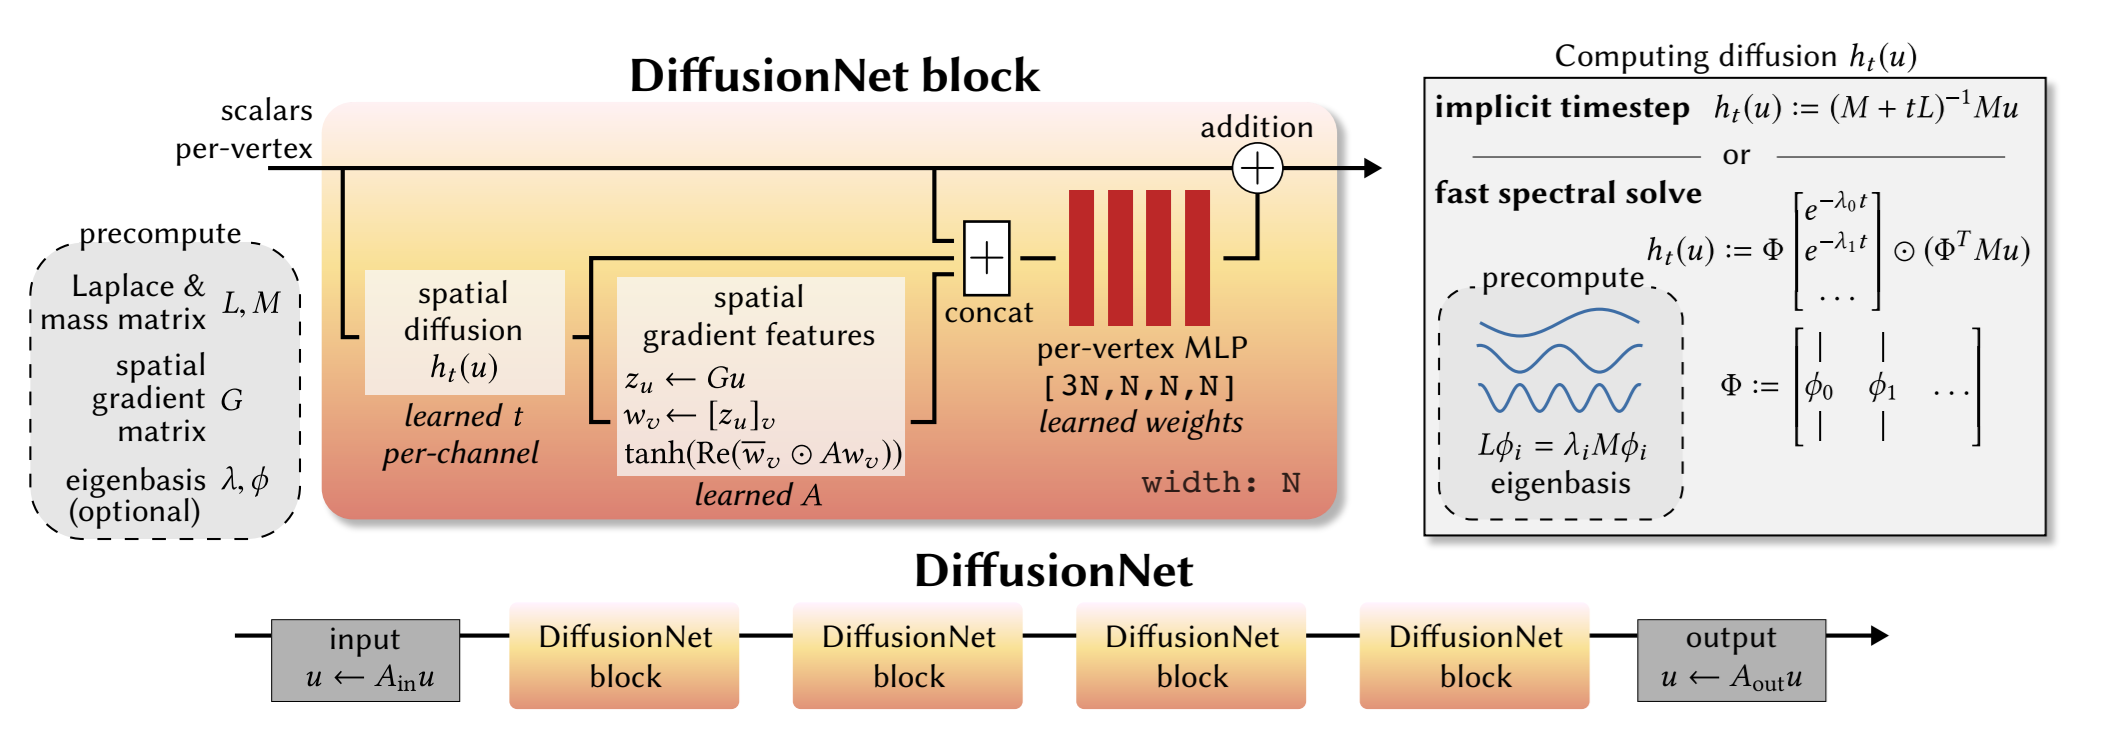
\includegraphics[width=1.0\textwidth]{images/diffusion-net.png}

\begin{itemize}
    \item A {\bf DiffusionNet architecture} is composed of several {\bf DiffusionNet blocks}.
    
    \item A DiffusionNet block starts with diffusion of input features, computation of spatial gradient features and then followed by per-point feature transformation with an MLP. The result is then added to the incoming features like what is done in ResNet.
    
    \item There is no need for spatial convolution or pooling on surfaces. 
\end{itemize}


\bibliographystyle{arxivalpha}
\bibliography{diffusion-net}  
\end{document}